\documentclass[main.tex]{subfiles}
\begin{document}

\chapter{Confidence Intervals and the Pivotal Quantity Method}\label{ch:guven}\chaptermark{Confidence Intervals}

A point estimate on its own is an incomplete answer: the value $\hat\theta=3.2$ does not say whether the uncertainty is $\pm0.1$ or $\pm5$. A confidence interval\index{confidence interval@confidence interval} is the frequentist way of reporting an estimate together with its uncertainty: in the long run, $95\%$ of the intervals constructed by the same method cover the true parameter. In this chapter we discuss the two general methods for constructing confidence intervals (pivotal\index{pivot@pivot} quantities and the inversion of tests), the basic results of normal sampling theory, and why the ``textbook'' Wald interval\index{wald confidence interval@Wald confidence interval} for a binomial proportion is surprisingly bad.

\section{Definitions}

\begin{definition}[Confidence Set and Confidence Coefficient]
Let $C(\X)\subseteq\Theta$ be a set depending on the data. $\P_\theta(\theta\in C(\X))$ is the \emph{coverage\index{coverage probability@coverage probability} probability} at $\theta$. If
\[
\inf_{\theta\in\Theta}\P_\theta\big(\theta\in C(\X)\big)\ge1-\alpha ,
\]
then $C$ is called a \emph{confidence set} of level $1-\alpha$; the infimum on the left is the \emph{confidence coefficient}. If $\Theta\subseteq\R$ and $C(\X)=[L(\X),U(\X)]$, it is called a \emph{confidence interval\index{confidence interval@confidence interval}}.
\end{definition}

\begin{remark}[The Correct Interpretation]
It is the interval that is random, not the parameter. The statement ``the probability that the interval $[2.9,\ 3.5]$ contains $\theta$ is $0.95$'' is --- in the frequentist sense --- false: the observed interval either contains $\theta$ or it does not. The correct statement is: ``the method that produced this interval covers $\theta$ in $95\%$ of repeated samples.'' A probability statement about the parameter is given by a Bayesian credible interval\index{credible interval@credible interval} (Chapter~\ref{ch:bayes}).
\end{remark}

\begin{definition}[Pivotal Quantity]\index{pivot@pivot|textbf}
A function $Q(\X,\theta)$ whose distribution does not depend on $\theta$ is called a \emph{pivot}. (It need not be a statistic; it involves $\theta$.) If its asymptotic distribution does not depend on $\theta$, it is called an \emph{asymptotic pivot}.
\end{definition}

\begin{definition}[The Chi-Square, Student $t$ and $F$ Distributions]\label{def:orneklem-dag}\index{t distribution student@$t$ distribution (Student)|textbf}
Let $Z,Z_1,\dots,Z_k\iid\Normal(0,1)$.
\begin{enumerate}
  \item $\sum_{j=1}^kZ_j^2\sim\chi^2_k$ (chi-square with $k$ degrees of freedom); $\chi^2_k=\text{Gamma}(k/2,\tfrac12)$ (rate $\tfrac12$), with mean $k$ and variance $2k$.
  \item If $V\sim\chi^2_k$ and $Z\indep V$, then $T=Z/\sqrt{V/k}\sim t_k$ (Student $t$).
  \item If $V_1\sim\chi^2_{k_1}$ and $V_2\sim\chi^2_{k_2}$ are independent, then $\frac{V_1/k_1}{V_2/k_2}\sim F_{k_1,k_2}$.
\end{enumerate}
The densities of these distributions are derived by the Jacobian\index{jacobian method@Jacobian method} method of Chapter~\ref{ch:ortak} (see Example~\ref{ex:beta-gamma} and the exercises there).
\end{definition}

\section{Normal Sampling Theory}

\begin{theorem}[The Normal Sample Theorem \cite{student08}]\label{thm:normal-orneklem}
If $X_1,\dots,X_n\iid\Normal(\mu,\sigma^2)$, then
\begin{enumerate}
  \item $\bar X\sim\Normal(\mu,\sigma^2/n)$;
  \item $\bar X$ and $S^2$ are independent;
  \item $\dfrac{(n-1)S^2}{\sigma^2}\sim\chi^2_{n-1}$;
  \item $T=\dfrac{\bar X-\mu}{S/\sqrt n}\sim t_{n-1}$.
\end{enumerate}
\end{theorem}
\begin{proof}
(1) A linear combination of independent normals is normal (Example~\ref{ex:normal-kf}).
(2) Basu\index{basu s theorem@Basu's theorem}'s theorem (Example~\ref{ex:normal-basu}).
(3) $\sum_{i=1}^n\big(\frac{X_i-\mu}{\sigma}\big)^2=\frac{(n-1)S^2}{\sigma^2}+\big(\frac{\bar X-\mu}{\sigma/\sqrt n}\big)^2$. The left-hand side is $\chi^2_n$, the second term on the right is $\chi^2_1$, and by (2) the two terms are independent. In terms of MGFs, $(1-2t)^{-n/2}=M_{(n-1)S^2/\sigma^2}(t)\cdot(1-2t)^{-1/2}$, so $M_{(n-1)S^2/\sigma^2}(t)=(1-2t)^{-(n-1)/2}$; this is the MGF of $\chi^2_{n-1}$.
(4) $T=\frac{(\bar X-\mu)/(\sigma/\sqrt n)}{\sqrt{[(n-1)S^2/\sigma^2]/(n-1)}}$; the numerator is $\Normal(0,1)$, and by (3) and the independence (2) the denominator has the form in the definition.
\end{proof}

\section{Methods for Constructing Confidence Intervals}

\begin{theorem}[The Pivot Method]\label{thm:pivot}\index{pivot@pivot}
Let $Q(\X,\theta)$ be a pivot and $a<b$ constants with $\P(a\le Q\le b)=1-\alpha$. Then $C(\X)=\{\theta: a\le Q(\X,\theta)\le b\}$ is an (exact) confidence set of level $1-\alpha$. If $Q$ is monotone in $\theta$, $C$ is an interval.
\end{theorem}
\begin{proof}
$\theta\in C(\X)\iff a\le Q(\X,\theta)\le b$; the probability of the right-hand side is $1-\alpha$ for every $\theta$.
\end{proof}

\begin{theorem}[Test--Interval Duality]\label{thm:dualite}\index{test interval duality@test--interval duality}
\begin{enumerate}
  \item For each $\theta_0\in\Theta$ let $A(\theta_0)$ be the acceptance region of a level-$\alpha$ test of $H_0:\theta=\theta_0$. Then
  \[
  C(\X) = \{\theta : \X \in A(\theta)\}
  \]
  is a confidence set of level $1-\alpha$.
  \item Conversely, if $C(\X)$ is a confidence set of level $1-\alpha$, then $A(\theta_0)=\{\x:\theta_0\in C(\x)\}$ is the acceptance region of a level-$\alpha$ test of $H_0:\theta=\theta_0$.
\end{enumerate}
\end{theorem}
\begin{proof}
Both directions rest on the identity $\theta\in C(\x)\iff\x\in A(\theta)$. Hence
\[
\P_\theta\big(\theta\in C(\X)\big)=\P_\theta\big(\X\in A(\theta)\big)=1-\P_\theta(H_0:\theta\text{ is rejected})\ge1-\alpha .\qedhere
\]
\end{proof}

\begin{remark}
Duality carries the optimality notions of test theory over to intervals: inverting UMP\index{uniformly most powerful ump test@uniformly most powerful (UMP) test} tests gives \emph{uniformly most accurate} confidence bounds, i.e.\ bounds with the smallest probability of covering false values $\theta'$. One-sided tests correspond to one-sided confidence bounds and two-sided tests to intervals.
\end{remark}

\begin{theorem}[The Shortest Pivotal Interval]\label{thm:en-kisa}\index{pivot@pivot}
Let the density $f$ of $Q$ be unimodal, and let the length of the interval be proportional to $b-a$. The interval minimising $b-a$ subject to $\int_a^bf=1-\alpha$ satisfies $f(a)=f(b)>0$ and $a\le x^*\le b$ ($x^*$: the mode). For symmetric $f$ this is the equal-tailed interval.
\end{theorem}
\begin{proof}
Unimodality: $f$ is non-decreasing on $(-\infty,x^*]$ and non-increasing on $[x^*,\infty)$. Let $[a,b]$ satisfy the conditions ($\int_a^bf=1-\alpha$, $f(a)=f(b)>0$, $a\le x^*\le b$); by unimodality $f\ge f(a)$ on $[a,b]$ and $f\le f(a)$ outside it. Suppose that some $[a',b']$ with $\int_{a'}^{b'}f\ge1-\alpha$ has $b'-a'<b-a$, and derive a contradiction.

\emph{Case 1: $a'\le a$.} Then $b'<b$.
(i) If $b'\le a$, then $f\le f(a)$ on $[a',b']\subseteq(-\infty,a]$ and
\[
\int_{a'}^{b'}f\le f(a)(b'-a')<f(a)(b-a)\le\int_a^bf=1-\alpha .
\]
(ii) If $a<b'<b$, then
\begin{align*}
\int_{a'}^{b'}f=\int_a^bf+\int_{a'}^{a}f-\int_{b'}^{b}f&\le(1-\alpha)+f(a)(a-a')-f(b)(b-b')\\
&=(1-\alpha)+f(a)\big[(b'-a')-(b-a)\big]<1-\alpha,
\end{align*}
because $f\le f(a)$ on $[a',a]$, $f\ge f(b)=f(a)$ on $[b',b]$, and $f(a)>0$.
In both subcases $\int_{a'}^{b'}f<1-\alpha$: a contradiction.

\emph{Case 2: $a'>a$.} The symmetric argument (Case~1 under the reflection $x\mapsto-x$) gives the same contradiction.

Hence $[a,b]$ is the shortest interval. If $f$ is symmetric about $0$, the choice $a=-b$ satisfies $f(a)=f(b)$ and the interval is equal-tailed.
\end{proof}

\section{Worked Examples}

\begin{example}[Normal Mean: The $t$ Interval]
The $T$ of Theorem~\ref{thm:normal-orneklem}(4) is a pivot\index{pivot@pivot}. Since $t_{n-1}$ is symmetric and unimodal, the shortest interval is
\[
\bar X\pm t_{n-1,\alpha/2}\frac{S}{\sqrt n} .
\]
If $\sigma$ were known, $z_{\alpha/2}$ would be used; the difference $t_{n-1,\alpha/2}>z_{\alpha/2}$ is the price of estimating $\sigma$ ($2.145$ vs $1.960$ for $n=15$).
\end{example}

\begin{example}[Normal Variance]
From the pivot $(n-1)S^2/\sigma^2\sim\chi^2_{n-1}$,
\[
\Big[\frac{(n-1)S^2}{\chi^2_{n-1,\alpha/2}},\ \frac{(n-1)S^2}{\chi^2_{n-1,1-\alpha/2}}\Big].
\]
Since the chi-square distribution\index{chi square distribution@chi-square distribution} is skewed, the equal-tailed interval is not the shortest (Theorem~\ref{thm:en-kisa}). Moreover, this interval is very sensitive to normality: if the excess kurtosis\index{kurtosis@kurtosis} $\gamma_2\ne0$, even the asymptotic coverage\index{coverage probability@coverage probability} is not $1-\alpha$ (because, by Theorem~\ref{thm:s2-yansiz}(3), $\Var(S^2)$ depends on $\mu_4$).
\end{example}

\begin{example}[Exponential Distribution]
$X_i\iid\text{Exp}(\lambda)$: $2\lambda\sum X_i\sim\chi^2_{2n}$ is a pivot. Hence
\[
\Big[\frac{\chi^2_{2n,1-\alpha/2}}{2\sum X_i},\ \frac{\chi^2_{2n,\alpha/2}}{2\sum X_i}\Big]
\]
is an exact $1-\alpha$ confidence interval\index{confidence interval@confidence interval} for $\lambda$.
\end{example}

\begin{example}[$\text{Uniform}(0,\theta)$]
The CDF of $Q=X_{(n)}/\theta$ is $q^n$ ($0<q<1$); it does not depend on $\theta$. Since the density $nq^{n-1}$ is increasing, the shortest interval is obtained with the choice $Q\in[\alpha^{1/n},1]$:
\[
\big[X_{(n)},\ X_{(n)}\alpha^{-1/n}\big].
\]
Its length is $O(1/n)$, faster than the $O(1/\sqrt n)$ of normal-based intervals.
\end{example}

\begin{example}[Binomial Proportion: Four Intervals]\label{ex:binom-ci}
$X\sim\text{Bin}(n,p)$, $\hat p=X/n$, $z=z_{\alpha/2}$.
\begin{enumerate}
  \item \textbf{Wald} (inverting the Wald test\index{wald test@Wald test}): $\hat p\pm z\sqrt{\hat p(1-\hat p)/n}$.
  \item \textbf{Wilson\index{wilson interval@Wilson interval}} \cite{wilson27} (inverting the score test\index{score rao test@score (Rao) test}): $\{p:\ |\hat p-p|\le z\sqrt{p(1-p)/n}\}$. Solving the quadratic inequality in $p$ gives
  \[
  \frac{\hat p+\frac{z^2}{2n}}{1+\frac{z^2}{n}}\pm\frac{z}{1+\frac{z^2}{n}}\sqrt{\frac{\hat p(1-\hat p)}{n}+\frac{z^2}{4n^2}}.
  \]
  \item \textbf{Clopper--Pearson\index{clopper pearson interval@Clopper--Pearson interval}} \cite{clopper34} (inverting exact binomial tests): the solutions of the equations $\P_p(X\ge x)=\alpha/2$ and $\P_p(X\le x)=\alpha/2$; in terms of Beta quantiles, $[B_{\alpha/2}(x,n-x+1),\ B_{1-\alpha/2}(x+1,n-x)]$.
  \item \textbf{Agresti--Coull\index{agresti coull interval@Agresti--Coull interval}} \cite{agresti98}: with $\tilde n=n+z^2$ and $\tilde p=(X+z^2/2)/\tilde n$, $\tilde p\pm z\sqrt{\tilde p(1-\tilde p)/\tilde n}$ (``add two successes and two failures'').
\end{enumerate}
These four intervals show how duality\index{test interval duality@test--interval duality} produces different intervals when different tests are applied to the same data. In the simulation below we shall see that the coverage of the Wald interval\index{wald confidence interval@Wald confidence interval} falls far below the nominal level at some values of $p$, even when $n$ is large \cite{brown-cai}.
\end{example}

\section{Computational Applications}

\subsection{Coverage of the $t$ Interval}

\pycode{code/ch16/c16_1_coverage_of_t_interval.py}
\begin{lstlisting}[style=output]
Coverage: 95.12%
with z instead (wrong): 93.12%
Normal | t-interval coverage=0.9501 | chi-square variance interval coverage=0.9506  (target 0.95)
Expon. | t-interval coverage=0.9118 | chi-square variance interval coverage=0.7430  (target 0.95)
\end{lstlisting}

For exponential data the $t$ interval for the mean gives reasonable coverage\index{coverage probability@coverage probability} even at $n=15$ (CLT\index{central limit theorem clt@central limit theorem (CLT)} and Slutsky\index{slutsky s theorem@Slutsky's theorem}), but the chi-square interval for the variance collapses: the excess kurtosis\index{kurtosis@kurtosis} of the exponential distribution is $6$.

\subsection{Binomial Proportion: Wald, Wilson, Clopper--Pearson, Agresti--Coull}
The coverage probabilities were computed exactly (by weighting with binomial probabilities).

\pycode{code/ch16/c16_2_binomial_wald_wilson_clopper_pearson.py}
\begin{lstlisting}[style=output]
n= 30 Wald             | mean coverage=0.8822 | min coverage=0.1396
n= 30 Wilson           | mean coverage=0.9527 | min coverage=0.8604
n= 30 Clopper-Pearson  | mean coverage=0.9731 | min coverage=0.9537
n= 30 Agresti-Coull    | mean coverage=0.9598 | min coverage=0.9339
n=100 Wald             | mean coverage=0.9288 | min coverage=0.3941
n=100 Wilson           | mean coverage=0.9511 | min coverage=0.9102
n=100 Clopper-Pearson  | mean coverage=0.9642 | min coverage=0.9504
n=100 Agresti-Coull    | mean coverage=0.9552 | min coverage=0.9391
n=100, p=0.01 | Wald=0.6334 | Wilson=0.9206 | CP=0.9816
n=100, p=0.05 | Wald=0.8775 | Wilson=0.9659 | CP=0.9826
n=100, p=0.20 | Wald=0.9331 | Wilson=0.9405 | CP=0.9674
n=100, p=0.50 | Wald=0.9431 | Wilson=0.9431 | CP=0.9648
\end{lstlisting}

\begin{figure}[h]
\centering
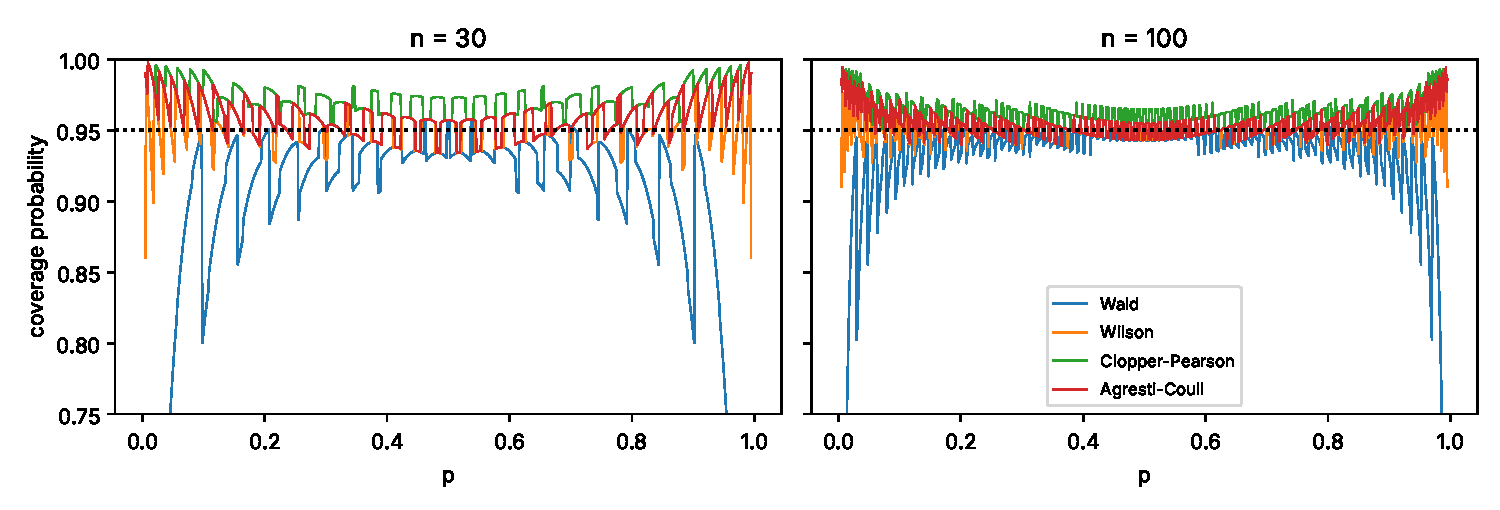
\includegraphics[width=\textwidth]{figures/binom_kapsama.pdf}
\caption{Exact coverage probabilities of $95\%$ intervals for a binomial proportion. The Wald interval (blue) gives dramatically low coverage, especially near the ends, and is erratic even at $n=100$. Clopper--Pearson is $\ge0.95$ everywhere (conservative); Wilson and Agresti--Coull are close to the nominal level on average.}
\end{figure}

\subsection{The Pivotal Interval for $\text{Uniform}(0,\theta)$}

\pycode{code/ch16/c16_3_uniform_pivotal_interval.py}
\begin{lstlisting}[style=output]
n=  5 | coverage=0.9502 | mean length=4.7865 | theory=4.7866
n= 20 | coverage=0.9495 | mean length=1.0773 | theory=1.0772
n=100 | coverage=0.9500 | mean length=0.2108 | theory=0.2108
\end{lstlisting}

\section{Comments and Notes}

\begin{remark}[Why Is the Wald Interval Bad?]
The Wald interval\index{wald confidence interval@Wald confidence interval} combines two approximations: the normal approximation \emph{and} evaluating the standard error at $\hat p$. When $p$ is near the ends, the distribution of $\hat p$ is skewed and $\hat p(1-\hat p)$ systematically underestimates the variance; moreover, when $\hat p\in\{0,1\}$ the interval collapses to a single point. The Wilson\index{wilson interval@Wilson interval} interval computes the variance at the value of $p$ under $H_0$ (the score approach) and avoids both problems. The general lesson: if the standard error of a parameter depends on that parameter, test inversion (score or LRT\index{likelihood ratio test lrt@likelihood ratio test (LRT)}) is more reliable than Wald.
\end{remark}

\begin{remark}[Why Are Exact Intervals Conservative?]
For discrete distributions, coverage\index{coverage probability@coverage probability} cannot be made exactly $1-\alpha$ without randomisation; Clopper--Pearson\index{clopper pearson interval@Clopper--Pearson interval} guarantees $\ge1-\alpha$ for every $p$ at the cost of intervals that are wider than necessary on average. This is the interval counterpart of the conservativeness of the non-randomised tests of Chapter~\ref{ch:neyman-pearson}.
\end{remark}

\begin{remark}[Bootstrap Intervals]
When no pivot\index{pivot@pivot} can be found and the asymptotic variance is complicated, the distribution of $\hat\theta$ can be imitated by resampling from the sample with replacement \cite{efron79}. The percentile\index{bootstrap@bootstrap!percentile interval@percentile interval}, BCa\index{bootstrap@bootstrap!bca interval@BCa interval} and bootstrap-$t$ intervals are data-driven versions of the pivot idea of this chapter; detailed theory and comparative simulations are in Chapter~\ref{ch:bootstrap}.
\end{remark}

% --- CHAPTER SUMMARY ---
\section{Chapter Summary}
\begin{summary}
\begin{itemize}
  \item In a confidence set it is the set, not the parameter, that is random. The coverage probability is the probability that the set contains the true parameter.
  \item The normal sample theorem (Theorem~\ref{thm:normal-orneklem}): $\bar X$ and $S^2$ are independent, $(n-1)S^2/\sigma^2\sim\chi^2_{n-1}$, and the studentised mean has a $t_{n-1}$ distribution.
  \item Intervals are constructed in two ways: the pivot method (Theorem~\ref{thm:pivot}) and test--interval duality (Theorem~\ref{thm:dualite}), i.e.\ inverting acceptance regions.
  \item For a unimodal pivot density, the shortest interval satisfies $f(a)=f(b)$ (Theorem~\ref{thm:en-kisa}). For symmetric pivots this interval is equal-tailed.
  \item For a binomial proportion the Wald interval gives very low coverage near the ends. The Wilson, Agresti--Coull and Clopper--Pearson intervals are more reliable.
\end{itemize}
\end{summary}
% --- END OF CHAPTER SUMMARY ---

\paragraph{Further reading.} \cite[Chapter~9]{casella}, \cite[Section~3.5 and Chapter~5]{lehmann-romano}; for a comparison of binomial intervals, \cite{brown-cai}.

\section{Exercises}

\begin{exercise}\label{exr:16-1}
For two independent normal samples ($\sigma_1=\sigma_2$ unknown), derive the pooled $t$ interval for $\mu_1-\mu_2$. If the variances are not equal, compare the coverage of the Welch \cite{welch47} approach by simulation.
\hfill\hyperref[coz:16-1]{\footnotesize$\rightarrow$\,Solution}
\end{exercise}

\begin{exercise}\label{exr:16-2}
For the interval for $\sigma^2$ based on the $\chi^2_{n-1}$ pivot, find the shortest interval by solving numerically the condition of Theorem~\ref{thm:en-kisa} (careful: the length is proportional to $(n-1)S^2(1/a-1/b)$!) and compare it with the equal-tailed interval for $n=10$.
\hfill\hyperref[coz:16-2]{\footnotesize$\rightarrow$\,Solution}
\end{exercise}

\begin{exercise}\label{exr:16-3}
For the Poisson mean $\lambda$, plot for $\lambda\in(0,\,5]$ the coverage of (a) the Wald interval, (b) the (inverted) score interval, and (c) the exact interval (Garwood: $\frac12\chi^2_{2x,1-\alpha/2}\le\lambda n\le\frac12\chi^2_{2x+2,\alpha/2}$).
\hfill\hyperref[coz:16-3]{\footnotesize$\rightarrow$\,Solution}
\end{exercise}

\begin{exercise}\label{exr:16-4}
$X_i\iid\Normal(\mu,\sigma^2)$. When the $t$ interval for $\mu$ and the chi-square interval for $\sigma^2$ are each constructed at level $95\%$, compute by simulation the probability that both are correct \emph{simultaneously}. Why is the result not $0.95^2=0.9025$, even though $\bar X\indep S^2$? (Hint: the coverage event of the $t$ interval also depends on $S$.) Construct a joint region with confidence at least $95\%$ using Bonferroni.
\hfill\hyperref[coz:16-4]{\footnotesize$\rightarrow$\,Solution}
\end{exercise}

\end{document}
